Το MIChartCard αποτελείται από ένα Grid το οποίο περιέχει ένα γράφημα Highcharts LineChart που στην ουσία είναι ένα γράφημα με μια η περισσότερες γραμμές, ένα εικονίδιο ακριβώς πάνω στο γράφημα περιγραφικό για τι δεδομένα παρουσιάζονται, και δεδομένα από κάτω. Τα δεδομένα του γραφήματος αναπτύσσουν ένα η παραπάνω ποσοτικό πεδίο ανά χρόνο για όσα χρόνια υπάρχουν στην συγκεκριμένη επιλεγμένη κατηγορία, ενώ τα δεδομένα από κάτω εμφανίζουν είτε τα μέγιστα, είτε τα ελάχιστα, είτε τους μέσους όρους των δεδομένων όπως φαίνεται στο σχήμα \ref{layout:michartcard}. Τα γραφήματα των MIChartCard Components όταν φιλτράρεται η κατηγορία ανά χρόνο απενεργοποιούνται, αλλά τα δεδομένα παρακάτω που αναγράφουν μέγιστα ελάχιστα και μέσους όρους παραμένουν και αναφέρονται στο επιλεγμένο έτος για αυτήν την κατηγορία. Δεν υπήρχε ουσιαστικός λόγος τα γραφήματα να έχουν δεδομένα καθώς αυτό που βλέπει ο χρήστης δεν είναι τα συνολικά δεδομένα παρά μόνο του επιλεγμένου έτους.

\begin{figure}[h]
  \centering
  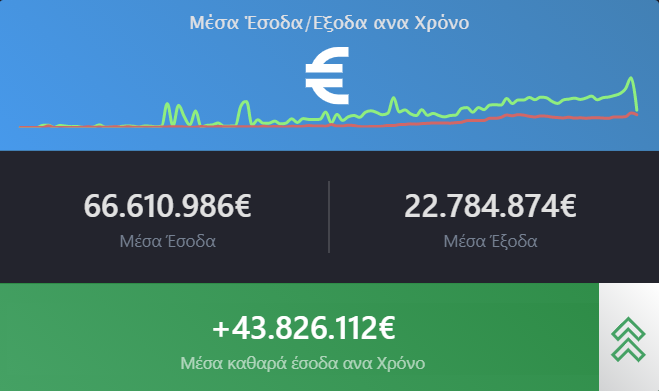
\includegraphics[width=80mm]{Chapters/5 - Architecture/Client/Images/michardcard.png}
  \caption{MIChartCard Component}
  \label{layout:michartcard}
\end{figure}